\documentclass[a4paper]{report}

%====================== PACKAGES ======================

\usepackage[french]{babel}
\usepackage[utf8x]{inputenc}
%pour gérer les positionnement d'images
\usepackage{float}
\usepackage{amsmath}
\usepackage{graphicx}
\usepackage[colorinlistoftodos]{todonotes}
\usepackage{url}
%pour les informations sur un document compilé en PDF et les liens externes / internes
\usepackage{hyperref}
%pour la mise en page des tableaux
\usepackage{array}
\usepackage{tabularx}
%pour utiliser \floatbarrier
%\usepackage{placeins}
%\usepackage{floatrow}
%espacement entre les lignes
\usepackage{setspace}
%modifier la mise en page de l'abstract
\usepackage{abstract}
%police et mise en page (marges) du document
\usepackage[T1]{fontenc}
\usepackage[top=2cm, bottom=2cm, left=2cm, right=2cm]{geometry}
%Pour les galerie d'images
\usepackage{subfig}

%====================== INFORMATION ET REGLES ======================

%rajouter les numérotation pour les \paragraphe et \subparagraphe
\setcounter{secnumdepth}{4}
\setcounter{tocdepth}{4}

\hypersetup{							% Information sur le document
pdfauthor = {Premier Auteur,
			Deuxième Auteur,
			Troisième Auteur,
    		Quatrième Auteur},			% Auteurs
pdftitle = {Nom du Projet -
			Sujet du Projet},			% Titre du document
pdfsubject = {Mémoire de Projet},		% Sujet
pdfkeywords = {Tag1, Tag2, Tag3, ...},	% Mots-clefs
pdfstartview={FitH}}					% ajuste la page à la largueur de l'écran
%pdfcreator = {MikTeX},% Logiciel qui a crée le document
%pdfproducer = {}} % Société avec produit le logiciel

%======================== DEBUT DU DOCUMENT ========================

\begin{document}

%régler l'espacement entre les lignes
\newcommand{\HRule}{\rule{\linewidth}{0.5mm}}

%page de garde
\begin{titlepage}
\begin{center}

% Upper part of the page. The '~' is needed because only works if a paragraph has started.

\includegraphics[width=0.35\textwidth]{./logo}~\\[1cm]

\textsc{\LARGE Université ou Entreprise}\\[1.5cm]

\textsc{\Large }\\[0.5cm]

% Title
\HRule \\[0.4cm]

{\huge \bfseries Nom du Projet\\
Sujet du Projet \\[0.4cm] }

\HRule \\[1.5cm]

% Author and supervisor
\begin{minipage}{0.4\textwidth}
\begin{flushleft} \large
\emph{Auteur:}\\
Premier \textsc{Auteur}\\
Deuxième \textsc{Auteur}\\
Troisième \textsc{Auteur}\\
Quatrième \textsc{Auteur}
\end{flushleft}
\end{minipage}
\begin{minipage}{0.4\textwidth}
\begin{flushright} \large
\emph{Client:} \\
Prénom \textsc{Nom}\\
\emph{Référent:} \\
Prénom \textsc{Nom}
\end{flushright}
\end{minipage}

\vfill

% Bottom of the page
{\large \today}

\end{center}
\end{titlepage}

%page blanche
\newpage
~
%ne pas numéroter cette page
\thispagestyle{empty}
\newpage

\renewcommand{\abstractnamefont}{\normalfont\Large\bfseries}
%\renewcommand{\abstracttextfont}{\normalfont\Huge}

\begin{abstract}
\hskip7mm

\begin{spacing}{1.3}

Lorem ipsum dolor sit amet, consectetur adipiscing elit. Sed non risus. Suspendisse lectus tortor, dignissim sit amet, adipiscing nec, ultricies sed, dolor. Cras elementum ultrices diam. Maecenas ligula massa, varius a, semper congue, euismod non, mi. Proin porttitor, orci nec nonummy molestie, enim est eleifend mi, non fermentum diam nisl sit amet erat. Duis semper. Duis arcu massa, scelerisque vitae, consequat in, pretium a, enim. Pellentesque congue. Ut in risus volutpat libero pharetra tempor. Cras vestibulum bibendum augue. Praesent egestas leo in pede. Praesent blandit odio eu enim. Pellentesque sed dui ut augue blandit sodales. Vestibulum ante ipsum primis in faucibus orci luctus et ultrices posuere cubilia Curae; Aliquam nibh. Mauris ac mauris sed pede pellentesque fermentum. Maecenas adipiscing ante non diam sodales hendrerit. Ut velit mauris, egestas sed, gravida nec, ornare ut, mi. Aenean ut orci vel massa suscipit pulvinar. Nulla sollicitudin. Fusce varius, ligula non tempus aliquam, nunc turpis ullamcorper nibh, in tempus sapien eros vitae ligula. Pellentesque rhoncus nunc et augue. Integer id felis. Curabitur aliquet pellentesque diam. Integer quis metus vitae elit lobortis egestas. Lorem ipsum dolor sit amet, consectetuer adipiscing elit. Morbi vel erat non mauris convallis vehicula. Nulla et sapien. Integer tortor tellus, aliquam faucibus, convallis id, congue eu, quam. Mauris ullamcorper felis vitae erat. Proin feugiat, augue non elementum posuere, metus purus iaculis lectus, et tristique ligula justo vitae magna. Aliquam convallis sollicitudin purus. Praesent aliquam, enim at fermentum mollis, ligula massa adipiscing nisl, ac euismod nibh nisl eu lectus. Fusce vulputate sem at sapien. Vivamus leo. Aliquam euismod libero eu enim. Nulla nec felis sed leo placerat imperdiet. Aenean suscipit nulla in justo. Suspendisse cursus rutrum augue. Nulla tincidunt tincidunt mi. Curabitur iaculis, lorem vel rhoncus faucibus, felis magna fermentum augue, et ultricies lacus lorem varius purus. Curabitur eu amet.

\end{spacing}
\end{abstract}


\tableofcontents
\thispagestyle{empty}
\setcounter{page}{0}
%ne pas numéroter le sommaire

\newpage

%espacement entre les lignes d'un tableau
\renewcommand{\arraystretch}{1.5}

%====================== INCLUSION DES PARTIES ======================

~
\thispagestyle{empty}
%recommencer la numérotation des pages à "1"
\setcounter{page}{0}
\newpage

\chapter{Présentation du projet}

Intro\footnotemark\\
%note en bas de page

\section{Sujet}

Bla(cf. fig. 1.1)\\

%inclusion d'une mage dans le document
\begin{figure}[!h]
\begin{center}
%taille de l'image en largeur
%remplacer "width" par "height" pour régler la hauteur
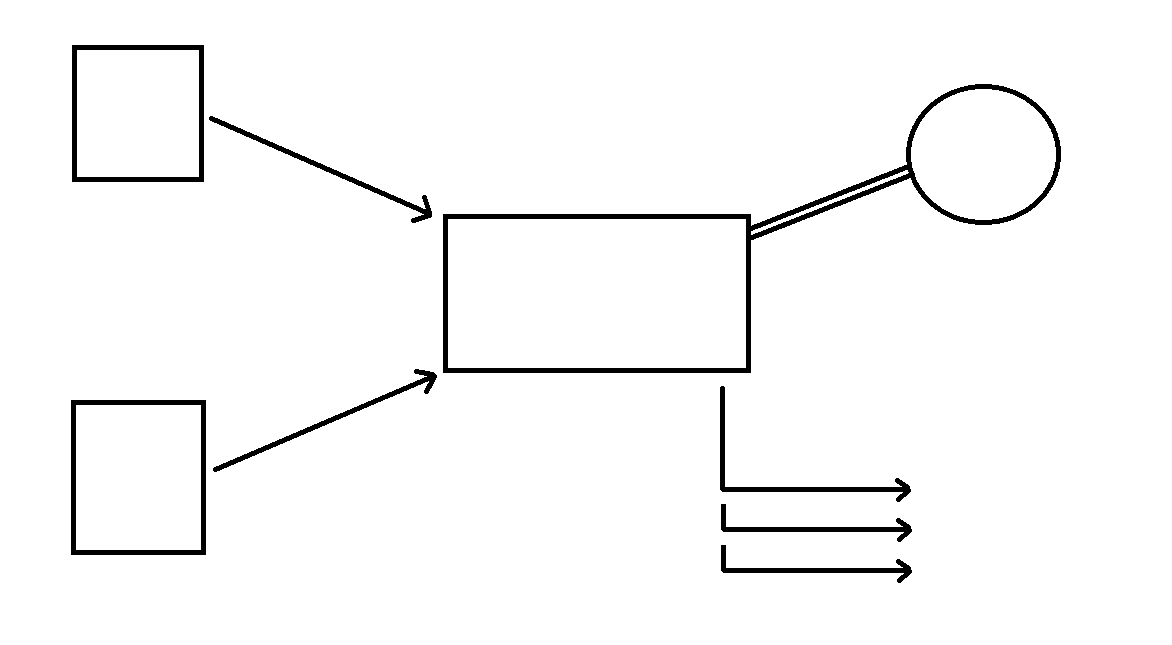
\includegraphics[width=15cm]{presentation/schema}
\end{center}
%légende de l'image
\caption{Schéma descriptif}
\end{figure}

%Contenu de la note précédemment marquée avec \footnotemark
\footnotetext{Note bas de page "intro"}

Bla
%retour à la ligne (alinea)

Bla\\
%saut de paragraphe

Bla

\newpage

\section{Problématique soulevée}

Bla

\begin{center}
Problématique du sujet
\end{center}

\section{Hypothèse de solution}

%Quoi :
Bla\\

Voici une liste :
\begin{itemize}
\item item 1;
\item item 2;
\item item 3;
\item item 4.
\end{itemize}

Bla\\

%Comment :
Bla

Bla\footnotemark\\

%Detail :
Bla(cf. ref. \cite{cite6}).
%citation référencé dans le document "bibliographie.bib" inclus à la fin du document

\footnotetext{Note bas de page "bla"}

\chapter{Analyse de l'existant}

Intro

\section{Partie 1}

Intro

\subsection{Sous-partie 1}

Bla

\subsection{Sous-partie 2}

Bla\\

Transition

\section{Partie 2}

Bla\\

Transition

\section{Bilan récapitulatif}

Voici un tableau (cf. fig. 2.1) récapitulatif de notre analyse de l'existant...\\

%tableau centré à taille variable qui s'ajuste automatiquement suivant la longueur du contenu
\begin{figure}[!h]
\begin{center}
\begin{tabular}{|l|l|l|l|l|}
  \hline
  Solution & Critère 1 & Critère 2 & Critère 3 & Critère 4\\
  \hline
  Solution 1(cf. ref. \cite{cite0}) & Oui & Oui & Oui & Oui \\
  Solution 2(cf. ref. \cite{cite1}) & Oui & Oui & Oui & Non \\
  Solution 3(cf. ref. \cite{cite2}) & Oui (sauf telle chose) & Non & Non & Oui\\
  Solution 4(cf. ref. \cite{cite3}) & Oui& Non & Oui & Non\\
  Solution 5(cf. ref. \cite{cite4}) & Oui (uniquement ceux-ci) & Non & Oui & Non\\
  \hline
\end{tabular}
\end{center}
\caption{Tableau récapitulatif des solutions}
\end{figure}

 
\chapter{Analyse des besoins}

Intro

\section{Besoins fonctionnels}

Après une analyse des besoins fonctionnels du projet, nous avons défini deux sous catégories. D'un côté, les besoins [...], de l'autre, les besoins [...].

\subsection{Sous-partie 1}

Bla

\subsection{Sous-partie 2}

Bla

\newpage

\section{Besoins non-fonctionnels}

Comme précédemment, nous avons choisi de distinguer deux catégories pour les besoins non-fonctionnels. D'une part, nous avons les besoins non-fonctionnels pour les [...], et d'autre part ceux pour [...]. Nous avons aussi pris en compte les contraintes de développement, que nous détaillerons à la fin de cette partie.

\subsection{Sous-partie 1}

Bla\\

Aperçu du rendu souhaité :

\begin{figure}[!h]
\begin{center}
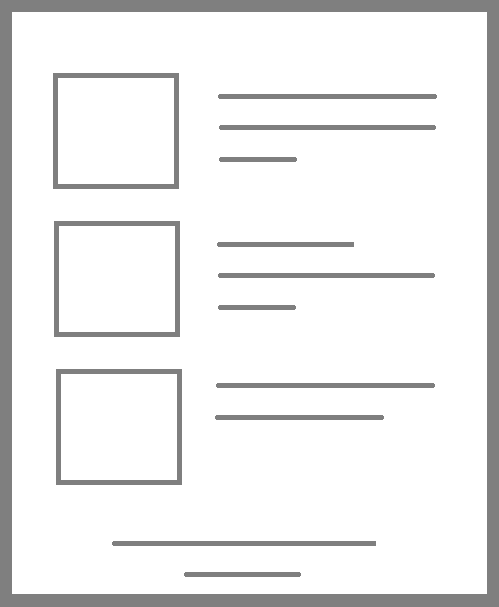
\includegraphics[height=10cm]{besoins/rendu}
\end{center}
\caption{Rendu attendu}
\end{figure}

\subsection{Sous-partie 2}

Bla

\newpage

\section{Développement}

Intro

\subsection{Tâches}

Bla\\


%tableau à taille fixée sur certaines colonnes (param sur la ligne \begin{tabularx}, voir wiki pour plus d'info sur la syntaxe
\begin{figure}[!h]
\begin{center}
\begin{tabularx}{17cm}{|c|p{6cm}|X|}
  \hline
  Priorité & Nom & Raison\\
  \hline
  1 & Tache 1 & Doit être vérifié en premier car sinon [...] \tabularnewline
  2 & Tache 2 & On doit pouvoir [...] \tabularnewline
  3 & Tache 3 & Comme les principales fonctionnalités permettant de tester sont opérationnelles, nous pouvons passer à cette tâche. \tabularnewline
  4 & Tache 4 & Parce que [...] \tabularnewline
  5 & Tache 5 & La tache 5 fait partie des principales [...]. \tabularnewline
  6 & Tache 6 & Dernière fonctionnalité essentielle à mettre en place. \tabularnewline
  7 & Tache 7 & Non-essentiel, mais apporterait un plus au projet. \tabularnewline
  8 & Tache 8 & Non-essentiel, mais apporterait un plus au projet. \tabularnewline
  \hline
\end{tabularx}
\end{center}
\caption{Tableau récapitulatif des tâches}
\end{figure}

\subsection{Tests}

Bla\\

\begin{figure}[!h]
\begin{center}
\begin{tabularx}{17cm}{|p{6cm}|X|}
  \hline
  Fonctionnalité & Test\\
  \hline
  Fonction 1 & Quand [...], vérifier [...]. \tabularnewline
  & Et quand [...], vérifier [...]. \tabularnewline
  Fonction 2 & Vérifier [...]. \tabularnewline
  Fonction 3 & Vérifier [...]. \tabularnewline
  Fonction 4 & Avoir [...]. \tabularnewline
  Fonction 5 & Accéder à [...]. \tabularnewline
   & Vérifier que [...]. \tabularnewline
  Fonction 6 & Accéder à [...]. \tabularnewline
   & Et vérifier [...]. \tabularnewline
  Fonction 7 & Installer [...]. \tabularnewline
   & Vérifier [...]. \tabularnewline
  Fonction 8 & Compter [...]. \tabularnewline
  \hline
\end{tabularx}
\end{center}
\caption{Tableau récapitulatif des tests}
\end{figure}

\chapter{Autre partie}

Dans cette partie nous cherchons à décrire dans un premier temps [...], puis, c[...].

\section{Partie 1}

Intro

\subsection{Sous-partie 1}

\begin{figure}[!ht]
\begin{center}

\includegraphics[height=12cm]{autre_partie/image1}
\end{center}
\caption[autre partie générale]{autre partie image 1\protect\footnotemark}
%\floatfoot{Source: (Citation command)}
% avec le package "floatrow"
\end{figure}

%footnote protected pour apparaitre dans la légende d'une image
\footnotetext{Schéma d'après : \textit{Auteur 1 \& Propriétaire image}, LICENCE (cf. ref. \cite{cite4})}

\newpage{}

\subsection{Sous-partie 2}

\begin{figure}[!ht]
\begin{center}

\includegraphics[height=12cm]{autre_partie/image2}
\end{center}
\caption[autre partie]{autre partie globale de notre quelque chose}
\end{figure}

Nous retrouvons ici, blabla\footnote{Application bla - Interface blabla} [...].

\subsubsection{Sous-sous-partie 1}

Le bla (cf. ref. \cite{cite6}) est [...]:

\begin{itemize}
\item item1;
\item item2;
\item item3;
\item item4;
\item item5.
\end{itemize}

\newpage

\subsubsection{Sous-sous-partie 2}

%Les lignes :
% \setcounter{secnumdepth}{4}
% \setcounter{tocdepth}{4}
%dans le fichier "main.tex" permettent de faire en sorte que les paragraphes soient interprété comme des titres de niveau 5
\paragraph{Paragraphe 1 (agissant comme titre niveau 5)}
%forcer un saut de ligne
~\\
\hskip7mm

\begin{figure}[!ht]
\begin{center}

\includegraphics[height=6cm]{autre_partie/image3}
\end{center}
\caption[Structure d'unz autre chose]{Structure d'une autre chose\protect\footnotemark}
\end{figure}

Ce schéma représente bla.

\footnotetext{Schéma et explication d'après le wiki bla (cf. ref. \cite{cite0})}

\paragraph{Paragraphe 2}
~\\
\hskip7mm

%fixer les floats précédemment définis
%\FloatBarrier

Bla

\subparagraph{Sous-paragraphe 1}
~\\
\hskip7mm

Bla

\begin{figure}[H]
\begin{center}

\includegraphics[height=10cm]{autre_partie/image4}
\end{center}
\caption{Diagramme de truc}
\end{figure}

\subparagraph{Sous-paragraphe 2}
~\\
\hskip7mm

Bla\\

Bla

\subparagraph{Sous-paragraphe 3}
~\\
\hskip7mm

Bla

\subsubsection{Sous-sous-partie 3}

Bla

\section{Partie 2}

Bla

\footnotetext{D'après le schéma disponible sur la documentfation officielle disponible sur le site blalbla}

Bla

\subsection{Sous-partie 1}

Bla

\subsection{Sous-partie 2}

Bla

\paragraph*{Paragraphe 1 (n'apparaitra pas dans l'index)}
Bla

\paragraph*{Paragraphe 2}
Bla

\paragraph*{Paragraphe 3}
Bla

\subsection{Sous-partie 3}

Bla

\chapter{Résultats}

\section{Partie 1}

Intro

\subsection{Sous-partie 1}

\paragraph*{Paragraphe 1 (n'apparaitra pas dans l'index)} Bla

\paragraph*{Paragraphe 2} Bla

\paragraph*{Paragraphe 3} Bla

\subsection{Sous-partie 2}

Bla

\subsection{Sous-partie 3}

Bla

\section{Partie 2}

Intro

\subsection*{Sous-partie 1 ('apparaitra pas dans l'index)} Bla

\paragraph*{Paragraphe 1 ('apparaitra pas dans l'index)} Bla

\paragraph*{Paragraphe 2} Bla

\paragraph*{Paragraphe 3} Bla

\newpage

\subsection*{Sous-partie 2}

Bla

%galerie d'image
\begin{figure}[htp]
  \centering
  \subfloat[Première image]{\label{fig:première}
\includegraphics[scale=0.8]{resultats/gallerie}}
  ~ %espace entre deux images sur une même ligne
  \subfloat[Deuxième image]{\label{fig:deuxième}
\includegraphics[scale=0.8]{resultats/gallerie}}
  ~
  \subfloat[Troisième image]{\label{fig:troisième}
\includegraphics[scale=0.8]{resultats/gallerie}}
  ~\\ %saute une ligne dans la galerie d'image
  \subfloat[Quatrième image]{\label{fig:quatrième}
\includegraphics[scale=0.8]{resultats/gallerie}}
  ~
  \subfloat[Cinquième image]{\label{fig:cinquième}
\includegraphics[scale=0.8]{resultats/gallerie}}
  \caption{Différents screenshots quelque chose, en gallerie}
  \label{fig:gallerie1}
\end{figure}

\chapter{Bilan}

%Rappel du context
Intro / Rappel Contexte

Nous avons donc pu en tirer la problématique suivante :

\begin{center}
\hskip7mm
Problématique du sujet
\end{center}

Bla

Bla\\

Bla\\

%Rappel des résultats
Bla

Bla\\

Bla

Bla

\newpage

%Conclusion/Perspectives
Bla

Bla\\

Bla

%Ne pas numéroter cette partie
\part*{Annexes}
%Rajouter la ligne "Annexes" dans le sommaire
\addcontentsline{toc}{part}{Annexes}

\chapter*{Annexe 1}
\addcontentsline{toc}{chapter}{Annexe 1}

%changer le format des sections, subsections pour apparaittre sans le num de chapitre
\makeatletter
\renewcommand{\thesection}{\@arabic\c@section}
\makeatother

%recommencer la numérotation des section à "1"
\setcounter{section}{0}

Intro

\section{Partie 1}

Bla

\subsection{Sous-partie 1}

Bla

\subsection{Sous-partie 2}

Bla

\subsection{Sous-partie 3}

Bla

\section{Partie 2}

Bla

\subsection{Sous-partie 1}

Bla

\subsection{Sous-partie 2}

Bla

\subsection{Sous-partie 3}

Bla

\chapter*{Annexe 2}
\addcontentsline{toc}{chapter}{Annexe 2}

%recommencer la numérotation des section à "1"
\setcounter{section}{0}

Intro

\section*{Prérequis}
\addcontentsline{toc}{section}{Prérequis}

Bla

\begin{itemize}
\item item1;
\item item2;
\item item3;
\item item4.
\end{itemize}

Bla

\section{Partie 1}

Bla

\subsection{Sous-parie 1}

Bla

\subsection{Sous-parie 2}

Bla

\section{Partie 2}

\begin{center}
\textsc{Attention !}

\textit{Texte d'avertissement}
\end{center}

Bla

\newpage

\section{Partie 3}

Bla

\begin{figure}[!ht]
\begin{center}
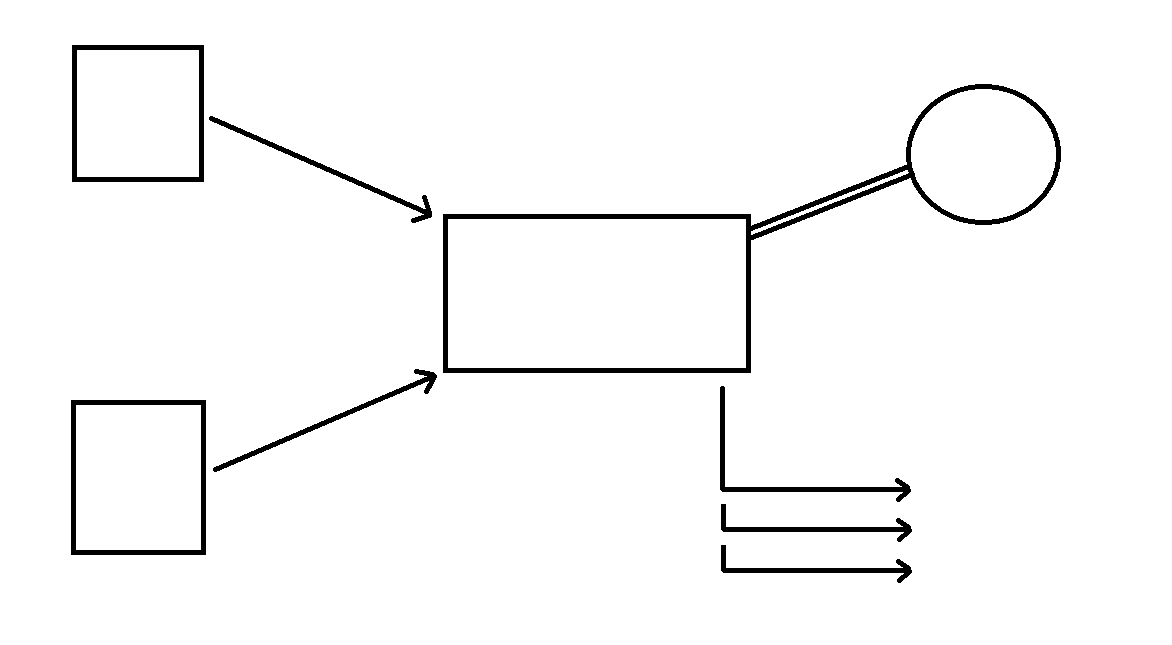
\includegraphics[height=8cm]{presentation/schema}
\end{center}
\caption[schema]{Presentation schema}
\end{figure}

\paragraph*{Paragraphe 1}
~\\
\hskip7mm

Bla

\paragraph*{Paragraphe 2}
~\\
\hskip7mm

Bla

\paragraph*{Paragraphe 3}
~\\
\hskip7mm

Bla

\newpage

%récupérer les citation avec "/footnotemark"
\nocite{*}

%choix du style de la biblio
\bibliographystyle{plain}
%inclusion de la biblio
\bibliography{bibliographie.bib}
%voir wiki pour plus d'information sur la syntaxe des entrées d'une bibliographie

\end{document}